%%%%%%%%%%%%%%%%%%%%%%%%%%%%%%%%%%%%%%%%%
%
% Igor D.C.
%
% igordc.com
%
% Official Curriculum Vitae,
% available at:
%
% https://github.com/igordcard/cv
%
% History and version tracking
% deferred to the git repository.
%
% All remaining credits are
% provided in the next block.
%
%%%%%%%%%%%%%%%%%%%%%%%%%%%%%%%%%%%%%%%%%

%%%%%%%%%%%%%%%%%%%%%%%%%%%%%%%%%%%%%%%%%
% Plasmati Graduate CV
% LaTeX Template
% Version 1.0 (24/3/13)
%
% This template has been downloaded from:
% http://www.LaTeXTemplates.com
%
% Original author:
% Alessandro Plasmati (alessandro.plasmati@gmail.com)
%
% License:
% CC BY-NC-SA 3.0 (http://creativecommons.org/licenses/by-nc-sa/3.0/)
%
% Important note:
% This template needs to be compiled with XeLaTeX.
% The main document font is called Fontin and can be downloaded for free
% from here: http://www.exljbris.com/fontin.html
%
%%%%%%%%%%%%%%%%%%%%%%%%%%%%%%%%%%%%%%%%%

%----------------------------------------------------
%	PACKAGES AND OTHER DOCUMENT CONFIGURATIONS
%----------------------------------------------------

\documentclass[letter,10pt]{article} % Default font size and paper size\usepackage{fullpage}

\usepackage{fontspec} % For loading fonts
\defaultfontfeatures{Mapping=tex-text}
\setmainfont[UprightFont = * Regular]{Fontin} % Main document font
\usepackage[top=0.75in, bottom=0.75in, left=1.0in, right=1.0in]{geometry}

\usepackage{xunicode,xltxtra,url,parskip} % Formatting packages
%\usepackage{url,parskip} % Formatting packages

\usepackage[usenames,dvipsnames]{xcolor} % Required for specifying custom colors

\usepackage{hyperref} % Required for adding links	and customizing them
\definecolor{linkcolour}{rgb}{0,0.2,0.6} % Link color
\hypersetup{colorlinks,breaklinks,urlcolor=linkcolour,linkcolor=linkcolour} % Set link colors throughout the document

\usepackage{titlesec} % Used to customize the \section command
\titleformat{\section}{\Large\scshape\raggedright}{}{0em}{}[\titlerule] % Text formatting of sections
\titleformat{\subsection}{\scshape\raggedright}{}{0em}{}[\titlerule] % Text formatting of subsections
\titlespacing{\section}{0pt}{3pt}{3pt} % Spacing around sections

\usepackage{multirow} % so I can put my avatar next to my Basic Data table


\begin{document}

\pagestyle{empty} % Removes page numbering

\font\fb=''[cmr10]'' % Change the font of the \LaTeX command under the skills section


%----------------------------------------------------
%	NAME AND CONTACT INFORMATION
%----------------------------------------------------

\par{\centering{\Huge Igor \textsc{D.C.}}\bigskip\par} % Your name

\section{Basic Data}

\begin{tabular}{rlr}
\textsc{Full name:} & Igor Duarte Cardoso & \multirow{9}{*}{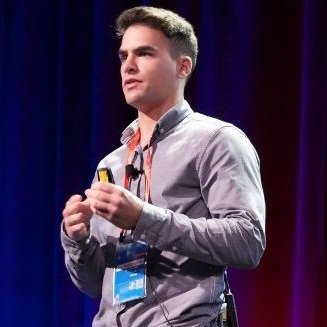
\includegraphics[scale=0.5]{avatar.jpg}} \\
\textsc{Degree:} & Master of Science in Computer and Telematics Engineering & \\
\textsc{Location:} & Clare, IRELAND & \\
\textsc{Origin:} & Leiria, PORTUGAL & \\
\textsc{Email:} & \href{mailto:igordcard+cv@gmail.com}{igordcard@gmail.com} & \\
% \textsc{Skype:} & \href{skype:igordcard?add}{igordcard}\\ % reactive Skype if externally available
\textsc{GitHub:} & \href{https://github.com/igordcard}{igordcard} & \\
\textsc{LinkedIn:} & \href{https://linkedin.com/in/igordcard}{igordcard} (not up-to-date) & \\
\textsc{Updated:} & 2018-September-12 (\textbf{Public Version}) & \\
\end{tabular} \\

%----------------------------------------------------
%	OBJECTIVES AND MOTIVATIONS
%----------------------------------------------------

\section{Objectives}

Having mostly worked in the fields of fields of Cloud Computing (IaaS), Software-Defined Networking (SDN) and Network Functions Virtualization (NFV), I'm always open to take on new challenges, leveraging parts of my experience and knowledge and applying that to other fields.

Both engineering and research interest me, and I have a tendency to enjoy design and architecture, including working with protocols (more on this in \nameref{section:work_experience}).

I want to take part in the evolution of existing (and development of new) technologies, learning and improving day after day. \\

%----------------------------------------------------
%	SKILLS
%----------------------------------------------------

\section{Skills}

\begin{tabular}{rl}
Basic Experience:
& Ansible, ASP.NET, bison, C, C++, Computer Architecture, Dansguardian, \\
& docker, flex, Google Analytics, iOS dev, Jekyll, Jenkins, MIPS assembly, \\
& Objective-C, OpenDaylight, OpenWrt, OSM, Perl, PHP, Public Speaking, \\
& Ruby, Squid3, x86 assembly, Intel RSD. \\
& \\
Intermediate Experience:
& Android dev, bash, C, C\#, Cisco IOS, CSS, ETSI NFV, Excel, git, \\
& GlassFish, GNS3, GNU/Linux, HTML, IETF SFC/NSH \\
& Intel Rack Scale Design, Java, JavaScript, JSON, LAMP, {\LaTeX}, \\
& Network Protocols, Neutron, OpenFlow, OpenStack, Open vSwitch, \\
& Python, Redfish, SQL, Technical Writing, UML, Vim, Visio, XML, Wireshark. \\
\end{tabular} \\

%----------------------------------------------------
%	INTERESTS AND ACTIVITIES
%----------------------------------------------------

\section{Interests and Activities}
Software\\
Cloud Computing\\
OpenStack\\
GNU/Linux\\
Open-Source\\
Computer Networks\\
Technology and Gadgets\\
Brainstorming\\
Health and Fitness\\
Brazillian Jiu-Jitsu\\
Reading\\

%----------------------------------------------------
%	WORK EXPERIENCE
%----------------------------------------------------

\section{Work Experience}
\label{section:work_experience}
\begin{tabular}{r|p{13.4cm}}

	\emph{Current} & Network Software Engineer \\
	\textsc{September 2015} & Intel Communications Europe (Shannon, Ireland) \\
	& \footnotesize{I have helped use cases and projects in the SDN, NFV and Orchestration areas on multiple occasions. Originally, I worked on the Group-Based Policy OpenStack project where I integrated QoS support from existing Neutron's APIs. Later, and during the majority of my time at Intel Communications Europe, I worked with SFC (Service Function Chaining). With a deep understanding of IETF SFC's proposal, architecture and the NSH protocol, I have fought through different obstacles in the OpenStack community in order to enable standards-compliant SFC, designing and proposing a compatible solution. I later implemented SFC Encapsulation support for OpenStack's Neutron (networking-sfc) through multiple patches, mainly the ones enabling Service Graphs and the NSH protocol (for Open vSwitch). Additionally, I have designed, developed and successfully contributed an abstract SFC interface for the VIM connector layer in the Open Source MANO (OSM) project, together with an OpenStack implementation of it, and enabled ETSI NSD/VNFFGD to be converted to the VIM connector's SFC interface, thus enabling top-to-bottom, end-to-end SFC from orchestration all the way down to Open vSwitch (optionally together with OpenDaylight), all based on open source projects. Another very significant endeavour was resurrecting the effort around traffic classification in OpenStack's Neutron, by founding and leading the Common Classification Framework project, creating an initial design and bringing the community together to discuss, suggest and agree on use cases and models. Most recently, I began working with Intel Rack Scale Design (RSD), where I have provided contributions on a diverse set of layers. My most tangible contribution in RSD is the inception of the \verb+rsb_+ module umbrella and the creation of the \verb+rsd_node+ module, allowing Ansible to deploy composed nodes in an idempotent manner. Finally, I've worked on multiple innovation tasks during my time.}\\
	\multicolumn{2}{c}{} \\

	\emph{September 2015} & Researcher and Software Engineer \\
    \textsc{October 2014} & Instituto de Telecomunicações (Aveiro, Portugal) \\
    & \footnotesize{Given the experience I acquired in OpenStack during my Master's Dissertation and the related work I did during it, I was invited to stay at Instituto de Telecomunicações doing research related to Network Functions Virtualization (NFV). There, I kept working on OpenStack although initially not upstream. Then started making contributions to the Group-Based Policy project for OpenStack. Most of my work, though, has been around other aspects of NFV: automating configuration of Virtual Network Functions (VNFs), improving and discussing the Traffic Steering implementation to meet the purposes of Service Function Chaining (SFC), testing and integrating other implementation artifacts of the team. }\\
	\multicolumn{2}{c}{} \\

	\emph{November 2015} & Developer, Designer and Marketeer \\
	\textsc{May 2013} & Wrkout (Aveiro, Portugal) \\
	& \footnotesize{Not really a job, but an amazing work experience. Wrkout is a mobile Android app which I've created. By dealing with multiple aspects related to developing, publishing and monetizing the app by myself, I have learned plenty. This project turned product also teaches me exactly why I should be working in a team. On November 2015 the app was made free and I became less engaged with it in order to better focus on my new endeavours.}\\
	\multicolumn{2}{c}{}\\

\end{tabular}

%----------------------------------------------------
%	ACHIEVEMENTS AND AWARDS
%----------------------------------------------------

\section{Achievements and Awards}

\begin{tabular}{rl}
    \textsc{2018} & Intel DSG DRA (Division Recognition Award) for my work in advancing IETF SFC and NSH. \normalsize\\
    \textsc{2017} & Intel DNSG DRA (Division Recognition Award) for my work in advancing IETF SFC and NSH. \normalsize\\
    \textsc{2016} & Founded the CCF for Neutron in OpenStack, successfully bringing the community together. \normalsize\\
    \textsc{2016} & Intel DNSG recognition for co-organizing the first ever OpenStack Days Ireland. \normalsize\\
    \textsc{2014} & Invited to develop a a mobile Android app (ActUA) by the University's top staff. \normalsize\\
    \textsc{2013} & First place on a University's Mobile App Development challenge awarded by Blip.pt. \normalsize\\
    \textsc{2011} & Research Integration1 Scholarship (12-month) at IEETA, financed by FCT. \normalsize\\
    \textsc{2008} & Top (\#1) High School finalist. \normalsize\\
\end{tabular} \\

%----------------------------------------------------
%	EDUCATION
%----------------------------------------------------

\section{Education}

\begin{tabular}{rl}
    \textsc{2014} & Master of Science in \textsc{Computer and Telematics Engineering}, \\
    &\textbf{Universidade de Aveiro}, Aveiro, Portugal, \\
    & Dissertation: ``Network Infrastructure Control for Virtual Campus'', \\
    & Integrated Master's includes both Bachelor's and Master's degrees: \\
    & Degree with a broad Computer Science foundation and multiple practical projects.\\
    & \textit{Final grade: 16 out of 20.}\\
    &\\

    \textsc{2008} & High School, \\
    &\textbf{Agrupamento de Escolas da Guia}, Guia, Portugal: \\
    & \textit{Final grade: 18 out of 20.}\\
    &\\
\end{tabular}

%----------------------------------------------------
%	MASTERS DISSERTATION
%----------------------------------------------------
\subsection{Master's Dissertation}
On my Master's Dissertation I have designed and developed an extension for OpenStack Neutron that allows virtually any computer network to be extended beyond their physical boundaries up to a Cloud-managed network, per a Cloud tenant's request. This is achieved through an architecture that uses pluggable drivers to communicate with remote devices that directly connect or manage these computer networks, automating all the process of reconfiguring them in order to extend their managed networks' broadcast domains up to the Cloud infrastructure (usually via some form of tunnelling). Examples of use cases that can be satisfied or made easier are: a) incrementally migrating legacy computer networks to the cloud; b) achieving the notion of a virtual campus, composed by multiple heterogeneous devices managed by the Cloud tenant or administrator, with virtual services deployed on top; c) on NFV, migrating current physical home gateways to a virtual home gateway environment, without replacing the customer's home gateway itself. Other use cases and in-depth coverage can be read on my publication: ``Seamless integration of Cloud and Fog networks'', referenced at the \nameref{section:publications} section.

%----------------------------------------------------
%	NON-FORMAL EDUCATION
%----------------------------------------------------
\subsection{Non-formal education}
\begin{itemize}
    \item Crucial Conversations and Conflict Resolution course (1 day).
    \item Public Speaking course (1 day).
\end{itemize}

%----------------------------------------------------
%	LANGUAGES
%----------------------------------------------------

\section{Languages}

\begin{tabular}{rl}
	\textsc{Portuguese:} & Native\\

	\textsc{English:} & Fluent\\

	\textsc{Spanish:} & Basic understanding\\

	\textsc{French:} & Basic understanding (if reading)\\

	\textsc{Italian:} & Basic understanding (if reading)\\
\end{tabular} \\

%----------------------------------------------------
%       PUBLICATIONS
%----------------------------------------------------

\section{Publications}
\label{section:publications}
\begin{tabular}{rl}
\textsc{2016} & Vitor Cunha, Igor D.C., J.P. Barraca, R.L. Aguiar: \\
& ``Policy-driven vCPE through dynamic network service function chaining''. \\
& NetSoft Conference and Workshops (NetSoft), 2016 IEEE, 156-160. \normalsize\\

\textsc{2016} & Igor D.C., J.P. Barraca, Carlos Goncalves, R.L. Aguiar: \\
& ``Seamless integration of Cloud and Fog networks''. \\
& International Journal of Network Management 26 (6), 435-460. \normalsize\\

\textsc{2015} & Igor D.C., J.P. Barraca, Carlos Goncalves, R.L. Aguiar: \\
& ``Seamless integration of Cloud and Fog networks''. \\
& 1st IEEE Conference on Network Softwarization (NetSoft 2015). \normalsize\\

\textsc{2014} & Paulo Dias, Tiago Sousa, Joao Parracho, Igor D.C., André Monteiro, Beatriz Sousa Santos: \\
& ``Student Projects Involving Novel Interaction with Large Displays''. \\
& IEEE Computer Graphics and Applications, vol. 34, no. 2, pp. 80-86, Mar.-Apr., 2014. \normalsize\\

\textsc{2014} & Tiago Sousa, Igor D.C., João Parracho, Paulo Dias, Beatriz Sousa Santos: \\
& ``DETI-Interact: Interaction with Large Displays in Public Spaces Using the Kinect''. \\
& HCI 2014 - 16th International Conference on Human-Computer Interaction: 196-206. \normalsize\\

\textsc{2014} & Igor D.C.: \\
& ``Network infrastructure control for virtual campuses''. \\
& Universidade de Aveiro (Master's Dissertation). \normalsize\\

\textsc{2013} & Tiago Sousa, João Parracho, Igor D.C., Paulo Dias, Beatriz Sousa Santos: \\
& ``Interação com ecrãs de larga dimensão usando o kinect''. \\
& Atas da 5ª Conferência Nacional sobre Interação-Interação. \normalsize\\

\textsc{2012} & Igor D.C., Paulo Dias, Beatriz Sousa Santos: \\
& ``Interaction with large displays in a public space using the Kinect sensor''. \\
& 20 Encontro português de Computação Gráfica - EPCG 2012, pp. 81–88 (2012). \normalsize\\

\end{tabular} \\

%----------------------------------------------------
%	PUBLIC PRESENTATIONS
%----------------------------------------------------

\section{Public Presentations}
\href{https://www.slideshare.net/igordcard/empower-your-nfv-services-through-service-function-chaining-and-sfc-graphs}{Empower your NFV Services through Service Function Chaining and SFC Graphs}\\
OpenStack Summit 2016, Barcelona

\href{https://www.slideshare.net/igordcard/developing-deploying-and-consuming-l47-network-services-in-an-openstack-cloud}{Developing, Deploying, and Consuming L4-7 Network Services in an OpenStack Cloud}\\
OpenStack Summit 2016, Austin

\href{https://www.slideshare.net/igordcard/cloud-sdn-nfv}{Cloud, SDN, NFV}\\
ENEI 2016, University of Aveiro, Portugal\\

I also voluntarily participate at my site's Lightning Talks from time to time.

%----------------------------------------------------
%	Open-Source Output
%----------------------------------------------------

\section{Open-Source Output}
I have made upstream contributions to a diverse set of projects within the OpenStack umbrella.

I have made other contributions to Open-Source software that are public but not all of them upstream, including irssi, Yakuake, metastore, tox, etc. I have also developed other simple side projects in the past, some of them available at my GitHub.

You can check most of my public output through the links/profiles/dashboards/pages below:
\begin{itemize}
    \item \href{https://review.openstack.org/#/q/owner:igordcard}{OpenStack Gerrit}
    \item \href{http://stackalytics.com/?user_id=igordcard&metric=marks&release=all}{OpenStack Stackalytics}
    \item \href{https://osm.etsi.org/gerrit/#/q/owner:cardosoi}{OSM Gerrit}
    \item \href{https://wiki.openstack.org/wiki/Neutron/CommonClassificationFramework}{CCF Wiki}
    \item \href{https://launchpad.net/~igordcard}{Launchpad Profile}
    \item \href{https://github.com/igordcard}{GitHub Profile}
\end{itemize}

%----------------------------------------------------
%	PRESENCE
%
% This section will deal with both my presence on the web (how to reach me, by professional profiles, etc)
% as well as my presence regardings groups, associations, development teams, open source projects, etc.
%----------------------------------------------------

\section{Presence}
\begin{tabular}{r|p{11cm}}
    \emph{ATNoG} & Advanced Telecommunications and Networks Group \\
    \textsc{September 2013} & \footnotesize{I became associated with ATNoG as part of my Master's Thesis. This group is established inside Aveiro's pole of Instituto de Telecomunicações.}\\
    \multicolumn{2}{c}{} \\
    \emph{GLUA} & University of Aveiro's Linux Group \\
    \textsc{July 2011} & \footnotesize{Member of the University of Aveiro's Linux Group (Grupo Linux da Universidade de Aveiro).}\\
    \multicolumn{2}{c}{}\\
\end{tabular}

%----------------------------------------------------
%	EVENTS
%----------------------------------------------------

\section{Events}
\begin{tabular}{r|p{11cm}}
    \emph{As a speaker and attendee} & OpenStack Summit 2016, Barcelona \\
     & OpenStack Summit 2016, Austin\\
     & ENEI 2016, University of Aveiro, Portugal\\
    \emph{As an attendee and meeting participant} & OpenStack Summit 2017, Boston \\
     & OpenStack PTG 2017, Atlanta \\
     & OpenStack Summit 2015, Tokyo \\
     & OpenStack Summit 2015, Vancouver \\
    \emph{As an attendee} & OpenStack Summit 2014, Paris \\
    \emph{As a co-organizer} & OpenStack Days Ireland 2016 \\
    \emph{As different roles} & Other events, conferences and challenges less related. \\
\end{tabular} \\

%----------------------------------------------------
%	PATENTS
%----------------------------------------------------

\section{Patents}
\begin{itemize}
    \item 1 Patent application, 2018, (title hidden until publicly available)
\end{itemize}

%----------------------------------------------------
%	ADDITIONAL NOTES
%----------------------------------------------------

%\section{Additional Notes}
%\begin{itemize}
%	\item Co-pioneer of <the box project> TODO add once ready
%\end{itemize}

\end{document}
